% Informe final: propagación sensorial en el conectoma de Drosophila
% Versión pública (sin matrícula). Compilar desde reporte/: latexmk -pdf informe-final.tex
\documentclass[11pt,letterpaper]{article}

\usepackage[T1]{fontenc}
\usepackage[utf8]{inputenc}
\usepackage{lmodern}
\IfFileExists{spanish.ldf}{%
  \usepackage[spanish,es-tabla,es-noshorthands]{babel}%
}{%
  \usepackage[english]{babel}%
  \addto\captionsenglish{%
    \renewcommand{\contentsname}{Índice}%
    \renewcommand{\refname}{Referencias}%
    \renewcommand{\figurename}{Figura}%
    \renewcommand{\tablename}{Tabla}%
    \renewcommand{\abstractname}{Resumen}}%
}
\usepackage[margin=2.5cm]{geometry}
\usepackage{microtype}
\usepackage{amsmath,amssymb}
\usepackage{booktabs,tabularx,array}
\usepackage{enumitem}
\usepackage[table]{xcolor}
\usepackage{graphicx}
\graphicspath{{../figuras/}{figuras/}}
\usepackage{caption}
\usepackage{float}
\usepackage{titlesec}
\usepackage{fancyhdr}
\usepackage[round,authoryear]{natbib}
\usepackage[hidelinks]{hyperref}

\definecolor{tinta}{HTML}{1F3A5F}
\definecolor{acento}{HTML}{B5432A}
\definecolor{suave}{HTML}{EEF2F6}

\titleformat{\section}{\large\bfseries\color{tinta}}{\thesection.}{0.6em}{}
\titleformat{\subsection}{\normalsize\bfseries\color{tinta}}{\thesubsection}{0.6em}{}
\setlist{itemsep=2pt,topsep=4pt}
\captionsetup{font=small,labelfont=bf}
\renewcommand{\arraystretch}{1.22}
\newcolumntype{L}{>{\raggedright\arraybackslash}X}
\newcolumntype{R}{>{\raggedleft\arraybackslash}X}

\pagestyle{fancy}
\fancyhf{}
\lhead{\small Informe final}
\rhead{\small Propagación sensorial en el conectoma de \emph{Drosophila}}
\cfoot{\small\thepage}
\renewcommand{\headrulewidth}{0.4pt}

\hypersetup{pdftitle={Informe final: propagación sensorial en el conectoma de Drosophila},
            pdfauthor={Atlahua Quiahuitl Martínez Obregón}}

\begin{document}

% ---------------------------------------------------------------- encabezado
\begin{center}
{\small Universidad Autónoma Metropolitana, Unidad Azcapotzalco · Ingeniería en Computación\par}
\vspace{0.5cm}
{\Large\bfseries\color{tinta} Informe final\par}
\vspace{0.15cm}
{\large Propagación sensorial en el conectoma de \emph{Drosophila}: del cerebro al cordón nervioso\par}
\vspace{0.4cm}
{\normalsize Atlahua Quiahuitl Martínez Obregón\par}
{\small Periodo: 17 al 21 de noviembre de 2026 · Entregado el sábado 21 de noviembre de 2026\par}
\vspace{0.2cm}
{\color{tinta}\rule{\linewidth}{0.6pt}}
\end{center}

\begin{abstract}
\noindent Se midió en cuántos pasos llega la información de cada modalidad sensorial a cada neurona de la mosca de la fruta y a sus motoneuronas, con el modelo de recorrido probabilístico de \citet{schlegel2021}, sobre dos conectomas públicos: el cerebro de FlyWire v783 y el cerebro con cordón nervioso del BANC v888. Una implementación propia, vectorizada y validada contra \texttt{navis}, reproduce las capas publicadas por \citet{dorkenwald2024} en las 13 modalidades (Spearman de 0.971 a 0.996), pero solo con el cerebro completo, sin umbral de sinapsis y con tope de 15 pasos. Los criterios para el BANC se fijaron antes de abrir sus datos. El orden de las capas por tipo celular se conserva entre las dos moscas (Spearman de 0.964 a 0.978): H2 se cumple. En el sistema nervioso completo, los mecanosensores de cada pata llegan a las motoneuronas de su propia pata de 1.5 a 2.1 pasos antes que la modalidad de la cabeza más cercana, unas 3 capas por encima de lo que dan 10 grafos al azar con los mismos grados. Pero el criterio fijado pedía 2 pasos en las tres patas y solo la pata trasera lo alcanza: H3 no se cumple tal como se planteó. El umbral de sinapsis cambia las capas (Spearman 0.88); el tope de pasos no. El código, las figuras y los resultados están en un repositorio público (v0.2).
\end{abstract}

% ---------------------------------------------------------------- 1
\section{Pregunta, hipótesis y estado final}

\begin{quote}
\emph{¿En cuántas capas del modelo de recorrido llega la información de cada modalidad sensorial a las motoneuronas de patas y alas, cuando se sigue el camino completo a través del cerebro y del cordón nervioso?}
\end{quote}

\begin{table}[H]
\centering
\small
\begin{tabularx}{\linewidth}{@{}p{2.9cm}Lp{3.2cm}@{}}
\toprule
\textbf{Pregunta} & \textbf{Criterio} & \textbf{Resultado} \\
\midrule
H1. Réplica & Spearman $\rho \ge 0.9$ por modalidad contra las capas publicadas & \textbf{Se cumple} (13 de 13) \\
H2. Dos moscas & Mediana de $\rho$ por tipo celular $\ge 0.7$ y al menos 3 de 4 modalidades $\ge 0.7$ & \textbf{Se cumple} (4 de 4) \\
H3. Atajo del cordón & En cada pata, sus mecanosensores llegan a sus motoneuronas al menos 2 pasos antes que la mejor modalidad de la cabeza, con IC 95\,\% sin 0 y mayor que en 10 grafos al azar; en las tres patas & \textbf{No se cumple} (solo T3) \\
P4. Sensibilidad & Sin hipótesis: mediana y rango de $\rho$ entre configuraciones & Umbral sí importa; tope no \\
\bottomrule
\end{tabularx}
\caption{Hipótesis del protocolo y resultado. Los criterios de H2, H3 y del control se escribieron en el plan el 20 de noviembre de 2026, a las 23:40, antes de abrir los datos del BANC, y no se cambiaron.}
\label{tab:estado}
\end{table}

\noindent Las cinco fases del plan se completaron entre el 17 y el 21 de noviembre. Repositorio público: \url{https://github.com/Quiwitl/fly-sensory-layers}, versión 0.2.

% ---------------------------------------------------------------- 2
\section{Datos}

\begin{itemize}
  \item \textbf{FlyWire v783.} Conexiones desde Zenodo (registro 10676866) y anotaciones de \citet{schlegel2024}. 139{,}262 neuronas, 15{,}091{,}983 pares conectados sin umbral (54.5 millones de sinapsis) y 2{,}700{,}513 pares con 5 sinapsis o más. Las cifras con umbral son iguales a las publicadas.
  \item \textbf{Capas publicadas.} Una tabla por modalidad con la capa media de cada neurona en 10{,}000 corridas \citep{rangos2024}.
  \item \textbf{BANC v888.} Desde Harvard Dataverse \citep{bancdata}: la lista de conexiones \texttt{simple\_v2} (11{,}752{,}828 pares sin umbral, la que usa \citealp{bates2026}) y las anotaciones (188{,}508 filas). Se quitan glía, elementos que no son neuronas y filas sin superclase. Para H2 quedan 122{,}575 neuronas y 7.72 millones de pares (cerebro: \texttt{central\_brain} y \texttt{optic\_lobe}); para H3, 146{,}769 neuronas y 10.65 millones de pares (sistema nervioso completo).
  \item \textbf{Semillas y blancos en el BANC.} Olfativas (3{,}007), gustativas de la cabeza (380), órgano de Johnston (1{,}193), proyección visual (7{,}316) y mecanosensores de pata delantera, media y trasera (1{,}322, 1{,}302 y 1{,}539). Blancos: motoneuronas de pata T1 (139), T2 (126), T3 (126) y de ala (64).
\end{itemize}

\begin{figure}[H]
\centering
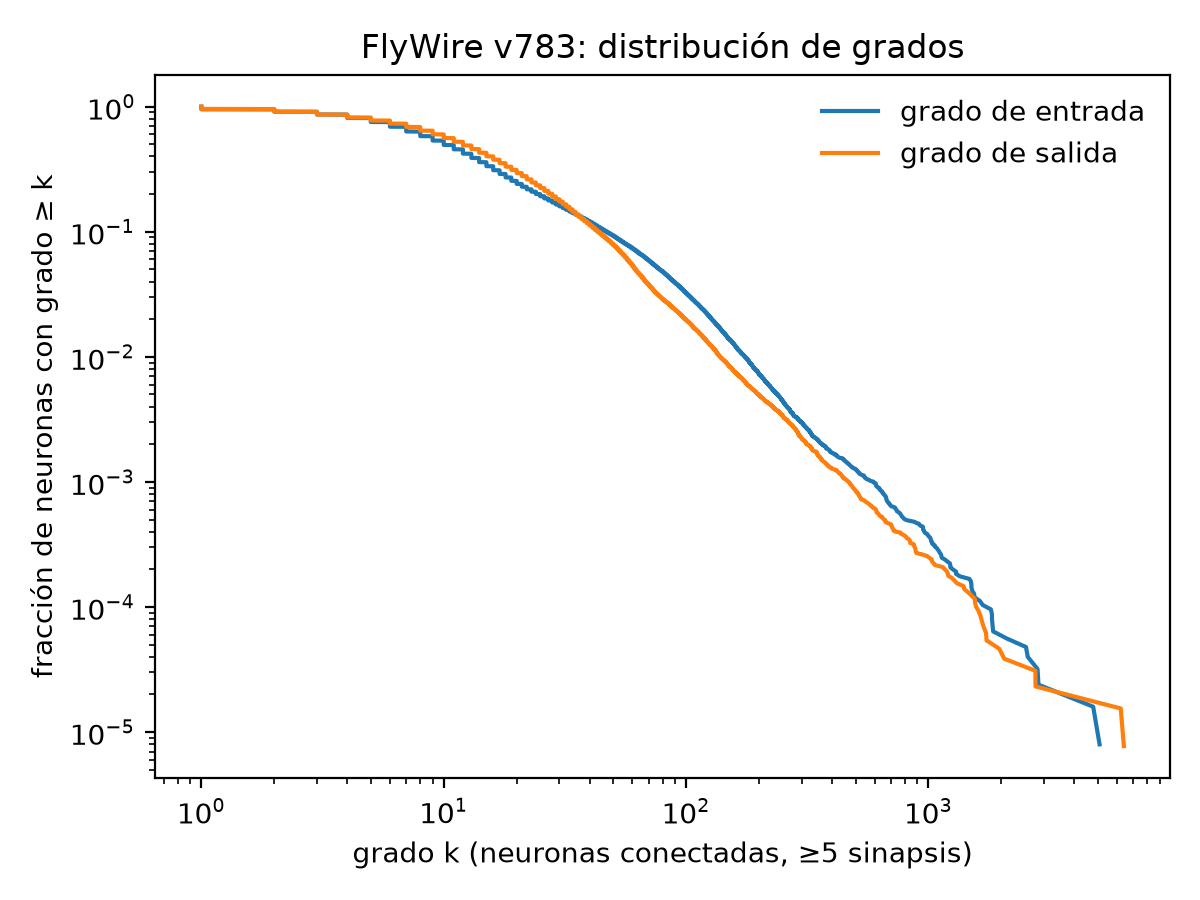
\includegraphics[width=0.5\linewidth]{01_grados.png}
\caption{Distribución de grados de FlyWire v783 (5 sinapsis o más).}
\end{figure}

% ---------------------------------------------------------------- 3
\section{Método}

\subsection{Modelo de recorrido}

Las neuronas semilla son la capa 1. En cada paso, cada arista $i\to j$ desde una neurona ya recorrida hacia una que no lo está tiene éxito con probabilidad
\[
p_{ij}=\min\!\left(1,\ \frac{A_{ij}}{0.3}\right), \qquad A_{ij}=\frac{W_{ij}}{\sum_k W_{kj}},
\]
donde $W$ es el número de sinapsis y $A$ la fracción de las entradas de $j$ que viene de $i$. La neurona $j$ entra si alguna de sus aristas tiene éxito, y su capa es ese paso. Una neurona que falla se vuelve a sortear en el paso siguiente. La corrida termina cuando no quedan aristas candidatas o al llegar al tope de pasos. La capa de cada neurona es el promedio sobre las corridas. Así lo hace \texttt{TraversalModel} de \texttt{navis} \citep{navis}.

\subsection{Implementación}

\begin{enumerate}
  \item \textbf{Un sorteo por neurona.} En lugar de sortear cada arista se sortea una vez por neurona con $P_j = 1-\prod_i(1-p_{ij})$, que tiene la misma distribución. El producto se calcula como $1-\exp\!\big(\sum_i \log(1-p_{ij})\big)$, que es un producto de matriz dispersa por el vector de neuronas recorridas.
  \item \textbf{Corridas en lote.} Cada corrida es una columna de una matriz densa, así que un paso de 100 corridas es una sola multiplicación dispersa por densa.
  \item \textbf{Regla de paro.} En FlyWire se agregan lotes de 100 corridas hasta que la capa media cambie menos de 0.01 en el 99\,\% de las neuronas (al menos 5 lotes). En el BANC se hacen siempre 1{,}000 corridas por modalidad.
  \item \textbf{GPU.} \texttt{recorrido\_gpu.py} hace lo mismo con CuPy \citep{cupy}: las matrices se copian a la tarjeta y cada paso es un producto de cuSPARSE. La regla de paro es la misma.
\end{enumerate}

\subsection{Validación}

\begin{itemize}
  \item \textbf{Pruebas.} 9 pruebas con grafos sintéticos (normalización, cadena, entrada de 30\,\% exacto, dirección, reproducibilidad, rapidez, regla por arista y reintento) y pruebas de propiedades.
  \item \textbf{Contra \texttt{navis}.} En un subgrafo de 1{,}610 neuronas, la diferencia media en las neuronas que no son semilla es de 0.001 capas.
  \item \textbf{GPU contra CPU.} En FlyWire, misma configuración y tres modalidades: $r \ge 0.999$, sesgo de 0.017 capas o menos y las mismas neuronas alcanzadas. En el BANC, el mismo grafo al azar en los dos motores: $r \ge 0.994$ y la medida de H3 igual a dos decimales.
\end{itemize}

\subsection{Análisis}

\begin{itemize}
  \item \textbf{H1.} Spearman entre la capa propia y la publicada por modalidad, sin semillas.
  \item \textbf{H2.} Capa media por tipo celular en FlyWire y en el cerebro del BANC, emparejando por \texttt{fafb\_cell\_type}; Spearman por modalidad de la cabeza, con tope de 15 pasos.
  \item \textbf{H3.} Capa mediana de las motoneuronas de cada pata desde cada modalidad, con tope de 30 pasos (también se reporta 15). Diferencia = capa desde la modalidad de la cabeza más cercana $-$ capa desde los mecanosensores de la pata; IC 95\,\% por bootstrap sobre motoneuronas (1{,}000 remuestreos).
  \item \textbf{Control.} 10 grafos al azar que conservan el grado de entrada y de salida de cada neurona, por intercambio de aristas \citep{maslov2002}: 10 rondas, unos 51.6 millones de intercambios por grafo, los 10.65 millones de pares se conservan. En cada grafo se repite el recorrido de H3.
  \item \textbf{P4.} Spearman de la capa media por neurona entre corridas de FlyWire que solo cambian el umbral (5 contra 1 sinapsis) o el tope (15 contra 30 pasos). Como referencia de ruido se comparan dos corridas de la misma configuración (CPU contra GPU).
\end{itemize}

% ---------------------------------------------------------------- 4
\section{Resultados}

\subsection{H1: réplica en FlyWire}

La primera comparación no cumplió H1 y la causa estaba en el grafo, no en el modelo. Los Métodos de \citet{dorkenwald2024} describen el cerebro central con umbral de 5 sinapsis, pero sus capas solo salen con otro grafo:

\begin{table}[H]
\centering
\small
\begin{tabularx}{\linewidth}{@{}LXX@{}}
\toprule
\textbf{Grafo} & \textbf{Spearman (13 modalidades)} & \textbf{Diferencia de capa} \\
\midrule
Cerebro central, $\ge 5$ sinapsis, 30 pasos & 0.65 -- 0.95 & hasta 1.4 capas \\
Cerebro completo, $\ge 5$ sinapsis, 15 pasos & 0.82 -- 0.95 & 0.06 a 1.2 capas más tarde \\
\textbf{Cerebro completo, sin umbral, 15 pasos} & \textbf{0.971 -- 0.996} & \textbf{0.05 -- 0.15 capas} \\
\bottomrule
\end{tabularx}
\caption{Réplica según el grafo, 1{,}000 corridas por modalidad. Solo la última configuración cumple H1.}
\end{table}

\noindent Tres pistas llevaron a esa configuración: la tabla publicada tiene unas 124 mil neuronas, más que el cerebro central (62 mil); con el cerebro completo las capas propias salían más tarde justo en las neuronas lejanas, como si faltaran caminos; y la capa máxima publicada es exactamente 15, el tope por defecto de \texttt{navis}. Por modalidad, el Spearman va de 0.971 (\emph{taste peg}) a 0.996 (fotorreceptores) y la diferencia media de capa de 0.05 a 0.15. Las neuronas olfativas alcanzan primero a las células de Kenyon olfativas y las de proyección visual a las Kenyon visuales, como se reporta.

\begin{figure}[tbp]
\centering
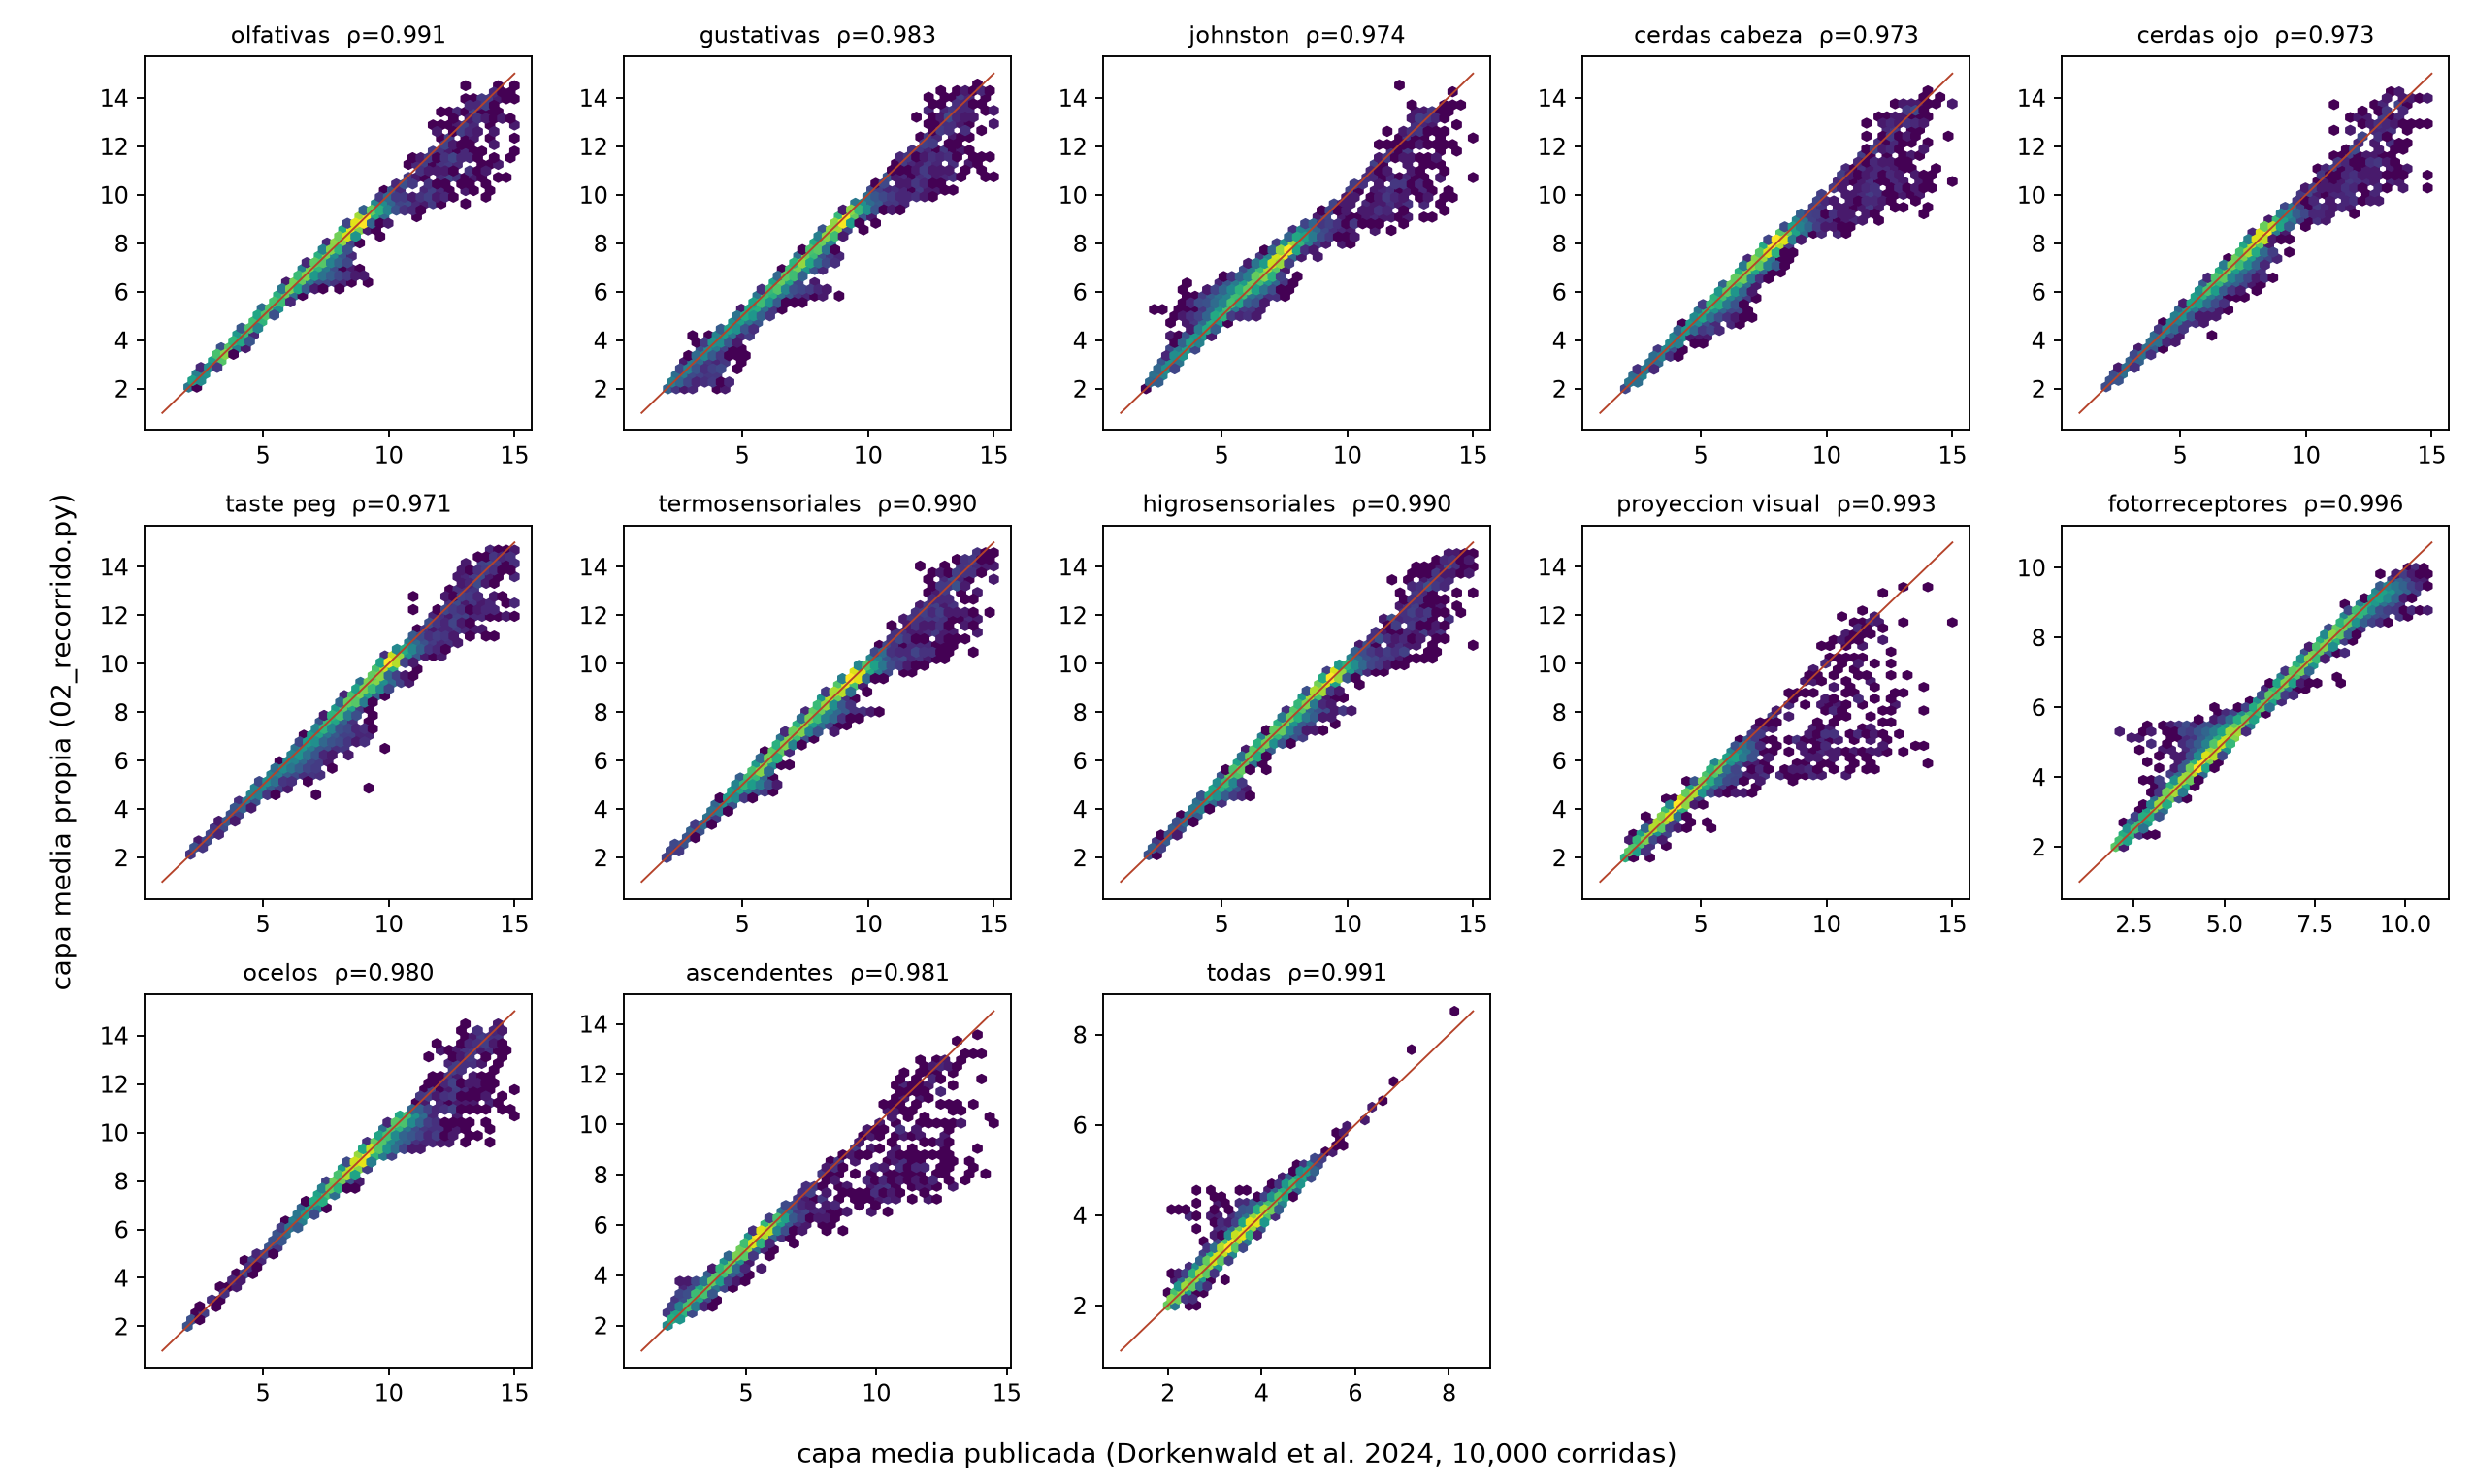
\includegraphics[width=0.92\linewidth]{03_propio_vs_publicado_completo_p15_u1.png}
\caption{Capa media propia contra publicada por modalidad (cerebro completo, sin umbral, 15 pasos). La línea roja es la igualdad.}
\end{figure}

\subsection{H2: el mismo orden en dos moscas}

\begin{table}[H]
\centering
\small
\begin{tabularx}{0.85\linewidth}{@{}LRR@{}}
\toprule
\textbf{Modalidad} & \textbf{Todos los tipos (7{,}528)} & \textbf{Tipos con $\ge 5$ neuronas (1{,}507)} \\
\midrule
Olfativas & 0.972 & 0.984 \\
Gustativas & 0.971 & 0.975 \\
Órgano de Johnston & 0.964 & 0.972 \\
Proyección visual & 0.978 & 0.985 \\
\midrule
Mediana & \textbf{0.971} & \textbf{0.980} \\
\bottomrule
\end{tabularx}
\caption{Spearman de la capa media por tipo celular entre FlyWire y el cerebro del BANC. H2 se cumple en las 4 modalidades.}
\end{table}

\noindent Sin semillas ni lóbulo óptico quedan 6{,}859 tipos, con Spearman de 0.967 a 0.975, y la diferencia mediana BANC $-$ FlyWire va de $-0.21$ a $+0.33$ capas. Como esperaba el protocolo, los tipos con más neuronas coinciden mejor.

\begin{figure}[H]
\centering
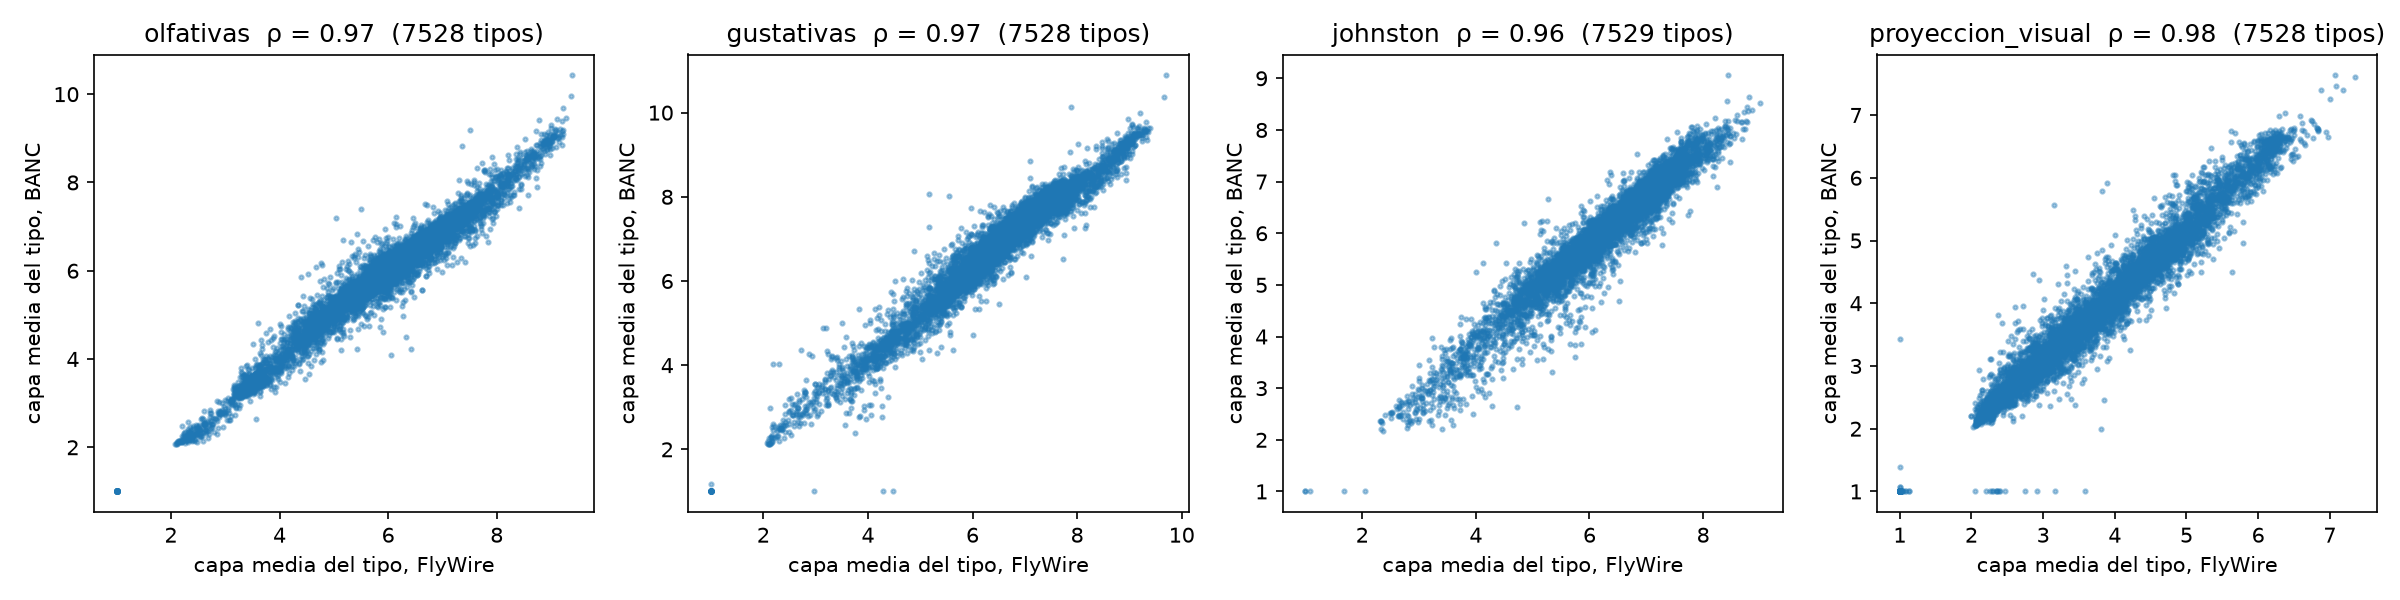
\includegraphics[width=\linewidth]{05_h2_tipos.png}
\caption{Capa media por tipo celular en FlyWire (eje horizontal) y en el BANC (eje vertical), por modalidad.}
\end{figure}

\subsection{H3: el atajo de las patas}

\begin{table}[H]
\centering
\small
\begin{tabularx}{\linewidth}{@{}LRRRR@{}}
\toprule
\textbf{Desde} & \textbf{MN pata T1} & \textbf{MN pata T2} & \textbf{MN pata T3} & \textbf{MN ala} \\
\midrule
Mecanosensores T1 & \textbf{3.95} & 5.38 & 5.67 & 5.94 \\
Mecanosensores T2 & 5.40 & \textbf{3.68} & 5.30 & 5.61 \\
Mecanosensores T3 & 5.69 & 5.34 & \textbf{3.56} & 5.65 \\
Proyección visual & 5.43 & 5.47 & 5.64 & 4.96 \\
Órgano de Johnston & 6.35 & 6.44 & 6.62 & 5.84 \\
Gustativas & 6.74 & 7.08 & 7.19 & 7.30 \\
Olfativas & 7.47 & 7.76 & 7.97 & 7.75 \\
\bottomrule
\end{tabularx}
\caption{Capa mediana de las motoneuronas (MN) de cada segmento desde cada modalidad, en el sistema nervioso completo del BANC (tope 30; con tope 15 sale igual, porque todas se alcanzan en el 100\,\% de las corridas).}
\end{table}

\noindent La diagonal se ve clara: los mecanosensores de cada pata llegan antes a las motoneuronas de su propio segmento que a las de las otras patas. De la cabeza, la modalidad más cercana a las patas es siempre la proyección visual, y la más lejana el olfato.

\begin{table}[H]
\centering
\small
\begin{tabularx}{\linewidth}{@{}p{1.2cm}XXp{2.2cm}p{2.6cm}@{}}
\toprule
\textbf{Pata} & \textbf{Grafo real (IC 95\,\%)} & \textbf{10 grafos al azar (rango)} & \textbf{¿Mayor que los 10?} & \textbf{¿Atajo según el criterio?} \\
\midrule
T1 & 1.48 (1.42 -- 1.53) & $-1.55$ a $-1.49$ & sí & no ($<2$ pasos) \\
T2 & 1.79 (1.74 -- 1.84) & $-1.26$ a $-1.22$ & sí & no ($<2$ pasos) \\
T3 & 2.08 (2.00 -- 2.12) & $-1.34$ a $-1.30$ & sí & \textbf{sí} \\
\bottomrule
\end{tabularx}
\caption{Diferencia = capa desde la proyección visual $-$ capa desde los mecanosensores de la pata. Con tope 15 sale igual.}
\label{tab:h3}
\end{table}

\noindent En los grafos al azar el signo se invierte: los mecanosensores quedan de 1.2 a 1.5 pasos \emph{más lejos} de las motoneuronas de su pata que la proyección visual, y los 10 grafos casi no varían entre sí (rango de 0.06 pasos o menos). Entonces la cercanía del grafo real, unas 3 capas por encima del azar, no la explica la distribución de grados: es cableado específico. Pero el criterio fijado pedía al menos 2 pasos en las tres patas, y T1 y T2 no llegan. \textbf{H3 no se cumple tal como se planteó.}

\begin{figure}[H]
\centering
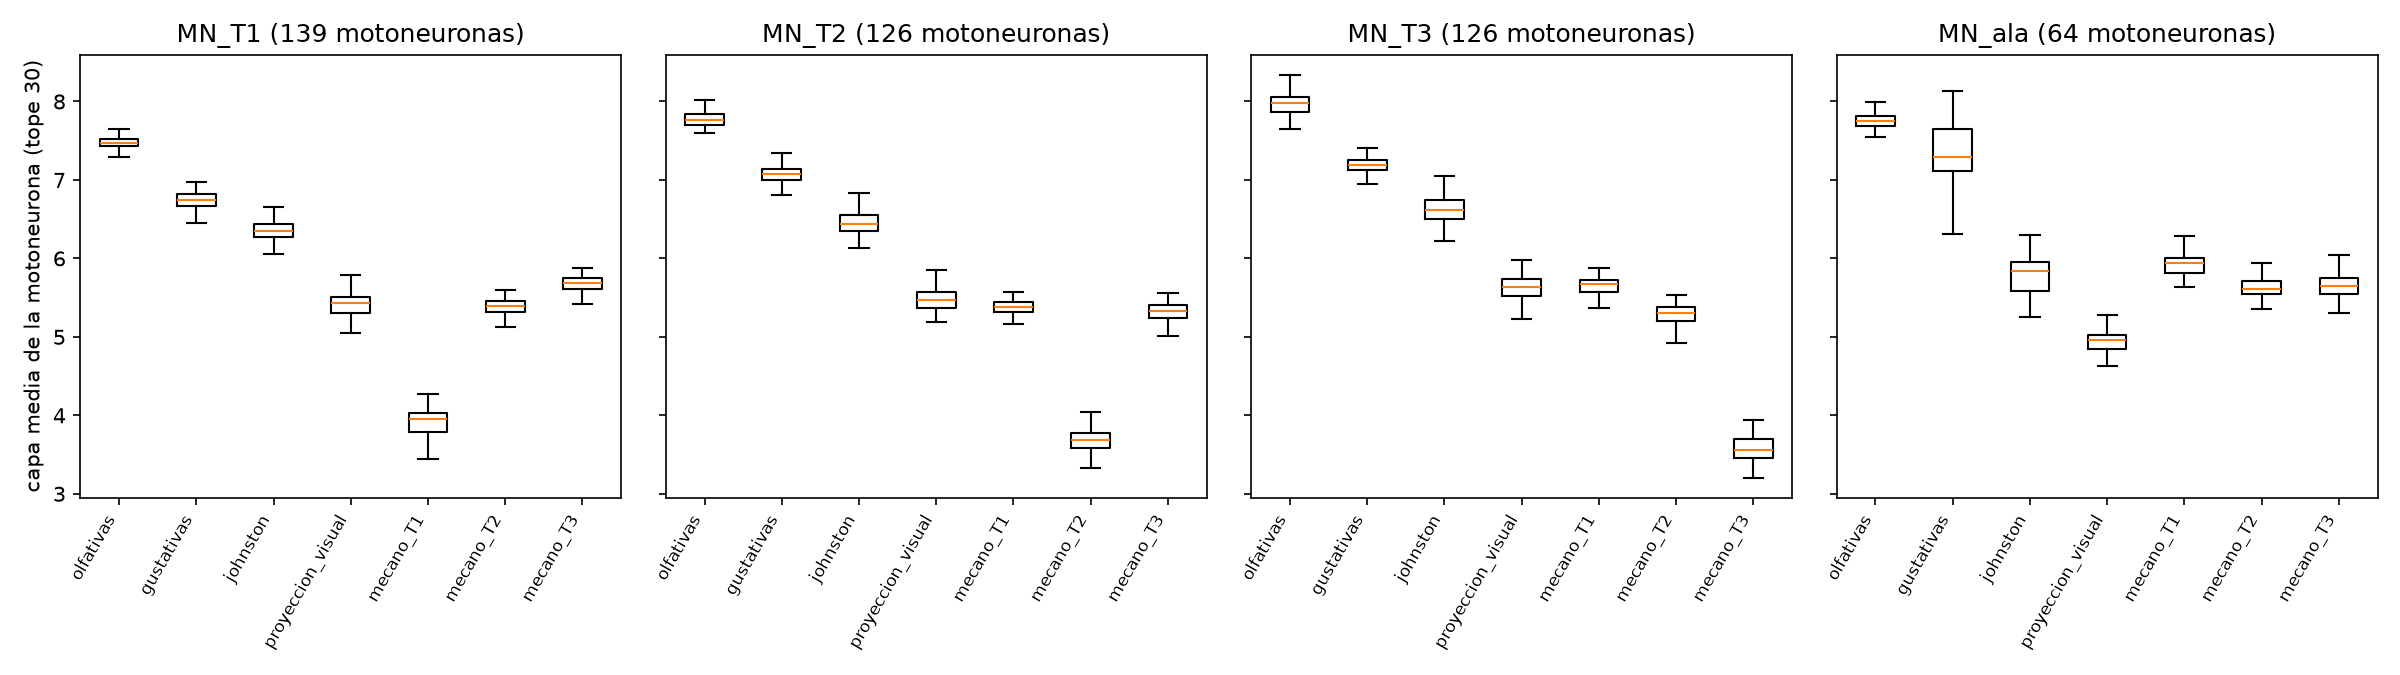
\includegraphics[width=\linewidth]{05_h3_motoneuronas.png}
\caption{Capa media de las motoneuronas de cada segmento desde cada modalidad (tope 30).}
\end{figure}

\subsection{P4: sensibilidad al umbral y al tope}

\begin{table}[H]
\centering
\small
\begin{tabularx}{\linewidth}{@{}Lp{1.7cm}p{2.5cm}L@{}}
\toprule
\textbf{Comparación} & \textbf{Mediana de $\rho$} & \textbf{Rango} & \textbf{Cambio de capa} \\
\midrule
Umbral: 5 contra 1 sinapsis (tope 15) & 0.880 & 0.837 -- 0.958 & sin umbral, de 0.07 a 1.25 capas antes; unas 12 mil neuronas más por modalidad \\
Tope: 15 contra 30 pasos (sin umbral) & 0.9985 & 0.9975 -- 0.9998 & 0.02 capas o menos; ninguna neurona nueva \\
Ruido: misma configuración, CPU contra GPU & 0.9971 & 0.9955 -- 0.9997 & 0.017 capas o menos \\
\bottomrule
\end{tabularx}
\caption{Spearman de la capa media por neurona en 12 modalidades de FlyWire, sin semillas. Las tres corridas de umbral y tope se hicieron en la GPU con la misma regla de paro (de 1{,}800 a 2{,}900 corridas por modalidad).}
\end{table}

\noindent El efecto del tope queda dentro del ruido. El del umbral no: las conexiones con menos de 5 sinapsis adelantan la llegada y suman neuronas. Las modalidades más afectadas son los ocelos y las cerdas del ojo.

\begin{figure}[H]
\centering
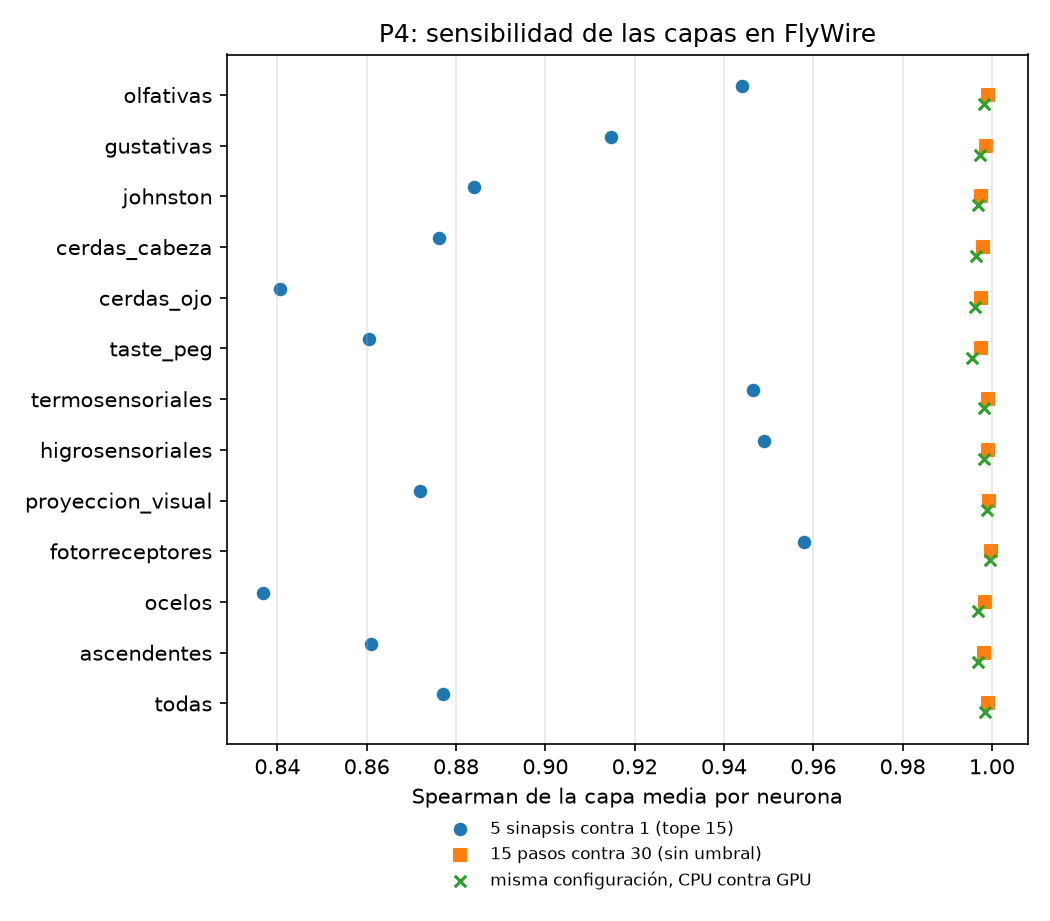
\includegraphics[width=0.75\linewidth]{06_sensibilidad.png}
\caption{Spearman por modalidad en cada comparación de P4.}
\end{figure}

% ---------------------------------------------------------------- 5
\section{Discusión}

\begin{enumerate}
  \item \textbf{Las conexiones débiles cuentan.} H1 y P4 dicen lo mismo desde dos lados: las capas publicadas solo se reproducen sin umbral, y quitar el umbral mueve las capas hasta 1.25 pasos. Las capas de recorrido de dos estudios solo se pueden comparar si usan el mismo umbral, y conviene reportarlo siempre junto con las capas. El tope de pasos, en cambio, no importa a partir de 15.
  \item \textbf{El orden de capas es del tipo celular, no del individuo.} Con dos moscas reconstruidas por equipos distintos, el orden se conserva con $\rho \approx 0.97$. Eso apoya usar la capa de recorrido como propiedad de cada tipo celular.
  \item \textbf{El atajo existe, pero es más chico de lo planteado.} Las tres patas tienen un camino a sus motoneuronas más corto que el de la cabeza y muy por encima del azar. Lo que no se cumple es el tamaño: 2 pasos era un umbral razonable, pero se eligió sin un antecedente que lo fijara. El resultado se reporta como salió; mover el umbral a 1.5 después de ver los datos haría que H3 se cumpliera, y por eso no se hace.
\end{enumerate}

\subsection{Limitaciones}

\begin{itemize}
  \item \textbf{H2 incluye el lóbulo óptico.} Casi todas las neuronas de proyección visual del BANC están anotadas en \texttt{optic\_lobe}; con solo \texttt{central\_brain} esa modalidad desaparece. La versión literal («cerebro sin cordón», solo cerebro central) queda en el código como opción.
  \item \textbf{Fracción de entrada dentro de cada subgrafo.} En H2 la fracción $A_{ij}$ se calcula sin las entradas que vienen del cordón, así que no es idéntica a la del sistema nervioso completo.
  \item \textbf{Corridas.} El BANC se corrió con 1{,}000 corridas por modalidad, sin regla de convergencia (cambio del último lote de 0.025 a 0.038 capas en el 99\,\% de las neuronas). Los intervalos de H3 son estrechos, así que no cambia el veredicto, pero las capas individuales tienen ese ruido.
  \item \textbf{Semillas.} Las gustativas del BANC son solo las de la cabeza; las de las patas quedan fuera para no mezclarlas con los mecanosensores.
  \item \textbf{Diferencia sin explicar.} Entre 15 y 17 mil neuronas tienen capa propia en FlyWire y no aparecen en la tabla publicada. No afecta los Spearman, porque solo se comparan neuronas presentes en ambas, pero falta saber por qué.
  \item \textbf{Un solo modelo.} Todo depende del modelo de recorrido y de su umbral de 0.3. No se compararon otras medidas de cercanía, como la influencia de \citet{bates2026}, porque ellos ya hicieron esa comparación.
\end{itemize}

% ---------------------------------------------------------------- 6
\section{Cambios respecto al protocolo}

\begin{table}[H]
\centering
\small
\begin{tabularx}{\linewidth}{@{}p{3.4cm}LL@{}}
\toprule
\textbf{Qué} & \textbf{Antes} & \textbf{Ahora y por qué} \\
\midrule
Grafo de H1 & Cerebro central, 5 sinapsis & Todo el cerebro, sin umbral, 15 pasos: es lo que reproduce lo publicado \\
Regla del modelo & Por neurona & Por arista, con reintento: es lo que hace \texttt{navis} \\
P4 & Recorrido contra la influencia del BANC & Sensibilidad al umbral y al tope: \citet{bates2026} ya compararon su influencia con el recorrido \\
Región de H2 & Cerebro sin cordón & \texttt{central\_brain} y \texttt{optic\_lobe}, para conservar la proyección visual \\
Corridas & 10{,}000 por modalidad & 1{,}000 en H1 y en el BANC; en P4, hasta converger (1{,}800 a 2{,}900) \\
Cómputo & CPU & GPU opcional, validada contra la CPU; el control y P4 se corrieron en la GPU \\
\bottomrule
\end{tabularx}
\caption{Desviaciones del protocolo y su justificación. Ninguna toca los criterios de H2, H3 ni del control.}
\end{table}

% ---------------------------------------------------------------- 7
\section{Reproducibilidad}

Todo se reproduce desde el repositorio con \texttt{uv}, que instala las dependencias de cada script:

\noindent\begin{minipage}{\linewidth}
{\small
\begin{verbatim}
uv run 00_descargar.py          # FlyWire, anotaciones, capas publicadas y BANC (con MD5)
uv run pruebas_recorrido.py     # pruebas del modelo
uv run 02_validar_navis.py      # contra navis
uv run 02_recorrido.py --alcance completo --umbral-sinapsis 1 \
       --max-pasos 15 --max-corridas 1000
uv run 03_validar_publicado.py _completo_p15_u1          # H1
uv run 04_banc.py --h2 ; uv run 04_banc.py --h3            # H2 y H3
uv run 04_azar_lote.py          # los 10 grafos al azar (--gpu para la GPU)
uv run 05_evaluar_banc.py       # H2, H3 y el control
python 02_recorrido.py ... --gpu --etiqueta _gpu          # tres corridas de P4
uv run 06_sensibilidad.py       # P4
\end{verbatim}
}
\end{minipage}
\medskip

\noindent Tiempos en una laptop de 16 hilos con una RTX 5050 de 8~GB: un grafo al azar del BANC tarda unos 31 minutos en CPU (4 procesos) y unos 6 en la GPU; una corrida completa de FlyWire, de 18 a 35 minutos en CPU y de 2 a 16 en la GPU. Los datos no se redistribuyen: FlyWire tiene licencia CC BY-NC 4.0; las capas publicadas y el BANC, CC BY 4.0. El código tiene licencia MIT.

% ---------------------------------------------------------------- 8
\section{Autoevaluación}

El protocolo se evaluó con la rúbrica \emph{Inquiry and Analysis} de la AAC\&U \citep{aacu2009} y con la de proyectos de investigación del CCH \citep{cchunam}, y dejó para este informe los criterios que necesitaban resultados.

\begin{table}[H]
\centering
\small
\rowcolors{2}{suave}{white}
\begin{tabularx}{\linewidth}{@{}p{3.1cm}Lc@{}}
\toprule
\textbf{Criterio} & \textbf{Evidencia en este informe} & \textbf{Nivel} \\
\midrule
Diseño & Criterios de H2, H3 y del control fijados antes de ver los datos; control contra el azar; validación del modelo en tres niveles & 4 \\
Análisis & Resultados organizados por hipótesis, con intervalos, control y referencia de ruido & 4 \\
Conclusiones & Se siguen de lo encontrado; H3 se reporta como no cumplida aunque el atajo exista & 4 \\
Limitaciones & Seis limitaciones concretas, con su efecto en los resultados & 3--4 \\
Redacción y citación & Clara y concisa; estilo \texttt{apalike}, parecido pero no idéntico a APA & 3 \\
\bottomrule
\end{tabularx}
\caption{Autoevaluación de los criterios que dependían de los resultados.}
\end{table}

% ---------------------------------------------------------------- 9
\section{Conclusiones}

Considero que el proyecto respondió su pregunta. La información sensorial llega a las motoneuronas de las patas en unos 3.5 a 4 pasos desde los mecanosensores de la misma pata, en unos 5.4 a 5.6 desde la visión y en casi 8 desde el olfato. El orden de las capas en el cerebro es estable entre dos moscas, y el atajo de las patas es real: está muy por encima del azar. Lo que no se cumplió fue el tamaño que yo mismo fijé para ese atajo, y prefiero reportarlo así que mover el criterio.

Lo que más aprendí no está en las hipótesis. Replicar un resultado publicado obligó a encontrar decisiones que el artículo no dice (el grafo completo, sin umbral, con tope de 15 pasos), y esas decisiones resultaron ser justo lo que más mueve las capas. También aprendí a fijar los criterios antes de ver los datos: sin eso, el resultado de H3 habría sido fácil de presentar como un éxito.

Queda abierto por qué 15 a 17 mil neuronas aparecen en las capas propias y no en las publicadas, y si el atajo de las patas cambia en otra mosca con cordón cuando haya otro conectoma completo.

\bibliographystyle{apalike}
\bibliography{referencias}

\end{document}
